\chapter{Einleitung}\label{sec:1_einleitung}
In diesem Kapitel wird die wissenschaftliche und praktische Motivation dieser Thesis dargelegt. Des Weiteren, wird der Projekt-Kontext dieser Arbeit erläutert um Hintergrund, Ziel und Abgrenzung dieser Arbeit besser verständlich zu machen.


\section{Motivation}\label{sec:1_motivation}
\ac{Ubicomp}, die Allgegenwart der virtuellen Welt in der Realität wird von vielen Designern erforscht \cite{Kuniavsky.2010}. Um Interaktion mit Systemen zu ermöglichen, ohne explizite \acp{UI} zu verwenden, werden neue Konzepte und Technologien benötigt. Seit Beginn des 21. Jahrhunderts hat sich \ac{IoT} als Schlüsselparadigma herauskristallisiert, um virtuelle und reale Welt verschmelzen zu lassen \cite{Gubbi.2013}. \ac{IoT}-Produkte reichen von Glühbirnen\footnote{\url{http://www.meethue.com}} die auf ihre Umgebung reagieren, bis hin zu intelligentem Besteck\footnote{\url{https://www.hapi.com/}}, welches das Essverhalten von Nutzern aufnimmt. Durch das Ausnutzen der digitalen Welt, haben sich Produkte auf dem Markt etabliert, welche die \ac{UX} ihrer analogen Vorgänger erweitern.

Obwohl die theoretischen Vorteile von intelligenten Objekten zahlreich sind, mangelt es oftmals noch an ihren praktischen Umsetzungen -- vor allem im Bereich der \ac{UX} \cite{Resnick.2013}. Diesem Umstand liegt die Tatsache zu Grunde, dass Produktentwicklung und Forschung im Bereich der \ac{IoT}, Designer und Wissenschaftler vor neue Herausforderungen stellt. Um die Effektivität neuer \ac{IoT}-Konzepte empirisch validieren zu können \cite{Robinson.2018}, benötigt es Prototypen, die diese Konzepte umsetzen. 

Das Entwickeln von \ac{IoT}-Prototypen, verlangt von Forschern und Designern, dass sie sich eine große Menge an technischem Fachwissen aneignen. Dieses Fachwissen lässt sich in zwei Teile auftrennen: 

\textbf{Erstens}, hardwarenahes Wissen (bspw. Elektrotechnik, Signalverarbeitung und Netzwerktechnik) um Komponenten und Infrastruktur der Prototypen bauen zu können. Diesem Problem nimmt sich \cite{weckbach2018cblocks} mit dem Werkzeug \acp{cBlock} an. \textbf{Zweitens} und Motivation dieser Thesis, ist das benötigte Wissen im Bereich des Software-Engineering und der Programmierung. \textit{Smart Objects} und \textit{connected Devices} können nur so intelligent sein, wie sie programmiert werden. Aus diesem Grund, muss sich der Designer intensiv mit der intrinsischen Komplexität der Programmierung und den Besonderheiten von hardwarenaher Programmierung auseinandersetzen. Diese zusätzliche Arbeitsbelastung ist nur bedingt zumutbar und erschwert die Erforschung von \ac{IoT}-Konzepten.

Das Aneignen dieses Wissens stellt eine Barriere für "`Nicht-Experten"' wie Designer dar. Allerdings besitzen diese "`Nicht-Experten"' gleichzeitig essentielles Wissen im Bereich der \ac{UX}. Es müssen daher Wege gefunden werden, diese Hürden zu nehmen oder zumindest so zu senken, dass eine iterativen Entwicklung von \ac{IoT}-Prototypen ohne tiefgründiges Fachwissen möglich ist. 

\section{Kontext}\label{sec:1_kontext}
Diese Thesis wird im Zusammenhang des zweijährigen Forschungsprojekts PROFI ("`Prototyping for Innovation"') geschrieben. Das Ziel des Projekts ist es, geeignete Werkzeuge zu erforschen, welche die Kommunikation zwischen Produkt-Entwicklung und Kunden durch den Einsatz von Prototyp-getriebener Entwicklung zu verbessern. Im Zuge dieses Projekts werden verschieden Prozesse, Software und Hardware entwickelt. Diese Komponenten sollen kleinen und mittelständischen Unternehmen bei der Erstellung von Prototypen im Bereich der \ac{IoT} helfen.

\begin{figure}[ht]
    \centering
    \begin{subfigure}[b]{0.3\textwidth}
        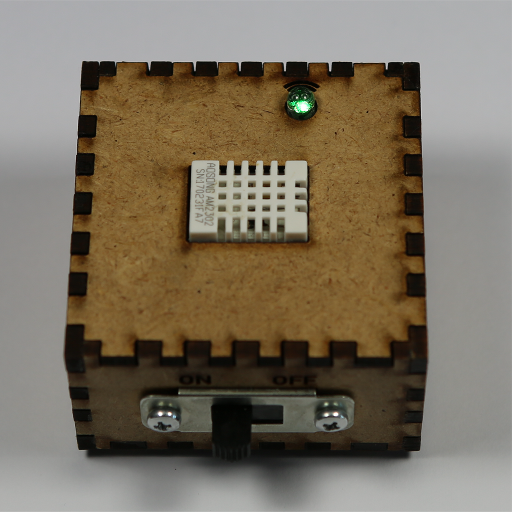
\includegraphics[width=1\linewidth]{bilder/chapter1/DHT22.png}
        \caption{}
        \label{fig:gull}
    \end{subfigure}
    \quad
    \begin{subfigure}[b]{0.3\textwidth}
        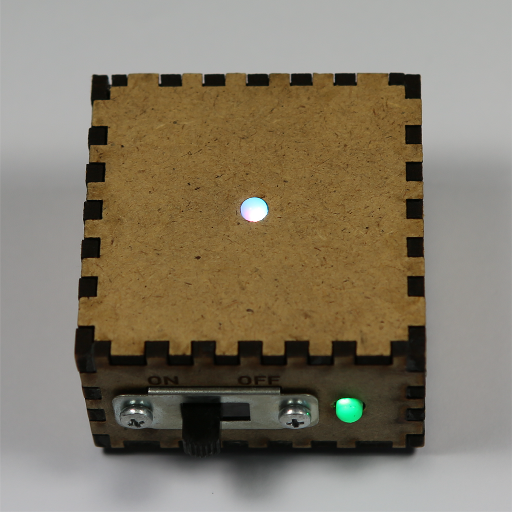
\includegraphics[width=1\linewidth]{bilder/chapter1/LED.png}
        \caption{}
        \label{fig:tiger}
    \end{subfigure}
    \quad
    \begin{subfigure}[b]{0.3\textwidth}
        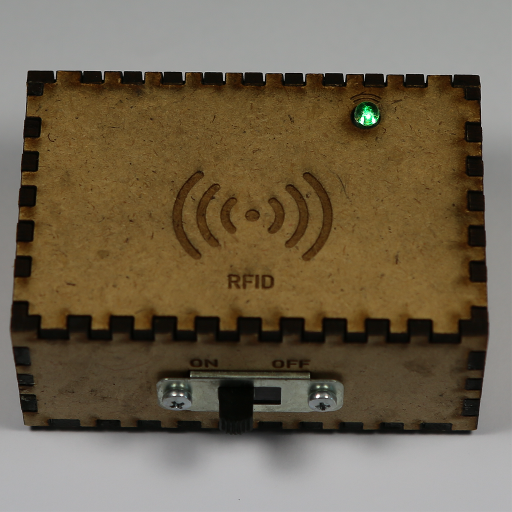
\includegraphics[width=1\linewidth]{bilder/chapter1/RFID.png}
        \caption{}
        \label{fig:mouse}
    \end{subfigure}
    \caption{Typische \acp{cBlock}. Hier bestehend aus drei unterschiedlichen Blöcken: Temperatur-Sensor (a),  LED-Aktor (b) und RFID-Sensor (c)}
    \label{fig:cblockfoto}
\end{figure}

Im Zuge dessen, wurde die Hardwareplattform \acp{cBlock} entwickelt. \acp{cBlock} ist ein \textit{Open-Source} Bausteinsystem zur Unterstützung von Designern beim Prototyping-Prozess von \ac{IoT} Produkten. Ein jeder Baustein abstrahiert verschiedenen Sensoren oder Aktoren und versucht dadurch, die Komplexität von hardwarenahen Entwicklungsaufgaben (bspw. Verdrahtung der Komponenten, Wählen von Protokollen, etc.) zu reduzieren. Das wichtigste Ziel von \acp{cBlock} ist allerdings nicht nur eine Aufwandsreduzierung auf Hardware-Ebene durchzuführen, sondern auch die Eintrittsbarriere für die Programmierung der Logik herunter zusetzen. Dadurch soll der technische Arbeitsaufwand von Designern so reduziert werden, dass sie sich darauf fokussieren können, neue \ac{IoT}-Erfahrungen zu erproben.

\section{Zielsetzung}\label{sec:1_zielsetzung}
Das \textbf{Ziel} dieser Thesis besteht darin, dem \textit{End-User}/Endnutzer (d.h. dem Designer) bei der Erstellung von Programmlogik, welche die \acp{cBlock} steuern, zu unterstützen. Hierfür wird eine \ac{EUD}-Plattform konzipiert und evaluiert, welche auf die Anforderungen der Domäne der \ac{IoT} sowie den Anforderungen der Endnutzer, gerecht wird. Dieses \ac{EUD}-Werkzeug, genannt \textit{flowws}, soll es Designern ermöglichen, zusammen mit den \acp{cBlock}, funktionale Prototypen zu gestalten.

Um dieses Ziel zu erreichen, sollen folgende Fragen beantwortet werden:
\begin{itemize}
    \item \textbf{\#1 Analyse \& Anforderung:} 
    \begin{itemize}
        \item Welche fundamentalen Probleme müssen \ac{EUD}-Werkzeuge in der \ac{IoT}-Domäne überwinden?
        \item Welche Anforderungen stellt die \ac{IoT} und die involvierten Stakeholder an ein \ac{EUD}-Werkzeug?
    \end{itemize}
        \item \textbf{\#2 Konzeption:} 
    \begin{itemize}
        \item Wie können die Eigenheiten der Anwendungsdomäne in ein \ac{EUD}-Konzept übertragen werden?
    \end{itemize}
        \item \textbf{\#3 Evaluation:} 
    \begin{itemize}
        \item Was sind die Vorteile des erarbeiteten Konzepts und inwiefern lassen sich die Erkenntnisse auf zukünftige Projekte ausweiten?
    \end{itemize}
\end{itemize}

\paragraph{Abgrenzung} Es ist nicht Ziel dieser Arbeit, ein \ac{EUD}-System für einen Produktiveinsatz (bspw. in Form einer Turing-vollständigen \ac{DSL}) zu konzipieren, sondern vielmehr eine geeignete Metaphern zu finden und \ac{UI}-Ansätze zu konzipieren und zu evaluieren, um einen besseren Einblick für zukünftige Projekte im Bereich des \ac{IoT}-Prototyping zu erhalten. Des Weiteren, grenzt sich diese Arbeit von ähnlichen Systemen wie bspw. eBlocks \cite{Phalke.2010} ab. Das zu erarbeitende Konzept legt den Anwendungsfokus nicht auf Bildung in der \ac{IoT}-Domäne. Es handelt sich bei flowws um ein Entwicklungswerkzeug, welches die Entwicklung von \ac{IoT}-Prototypen unterstützen soll.

\section{Aufbau der Arbeit}\label{sec:1_aufbau}
\begin{itemize}
    \item \textbf{Kapitel 2 Grundlagen und State-of-the-Art:} Hierbei werden die fundamentalen Aspekte der \ac{IoT}- und \ac{EUD}-Domäne diskutiert. Zusätzlich werden bestehende \acp{EUD}-Systeme mit vergleichbarem Fokus analysiert.
    \item \textbf{Kapitel 3 Anforderungen:} In diesem Abschnitt, werden Probleme von bestehenden \acp{EUD}-Systemen und die Stakeholder analysiert. Daraus abgeleitet, entstehen Vision und Ziele für das \ac{EUD}-Werkzeug, welche wiederum in Szenarios und Anforderungen transformiert werden.
    \item \textbf{Kapitel 4 Konzeption:} Die verschiedenen Aspekte des \ac{EUD}-Werkzeugs "`flowws"' wird in diesem Kapitel konzipiert.
    \item \textbf{Kapitel 5 Evaluation:} In diesem Kapitel wird das Konzeptmodell von flowws wird durch Nutzertests auf seine Verständlichkeit überprüft und die Ergebnisse analysiert.
    \item \textbf{Kapitel 6 Diskussion:} Zum Schluss werden die erarbeiteten Ergebnisse zusammengefasst, bewertet und einen Ausblick für zukünftige Arbeiten gegeben.
\end{itemize}